\documentclass{article}
\usepackage{../fasy-hw}
\usepackage{ wasysym }

%% UPDATE these variables:
\renewcommand{\hwnum}{7}
\title{Advanced Algorithms, Homework \hwnum}
\author{Kevin Browder \and Seth Bassetti \and Nathan Stouffer}
\collab{Kevin Browder, Seth Bassetti, Nathan Stouffer}
\date{due: 9 November 2020}

\begin{document}

\maketitle

This homework assignment should be submitted as a single PDF file to to Gradescope.

General homework expectations:
\begin{itemize}
    \item Homework should be typeset using LaTex.
    \item Answers should be in complete sentences and proofread.
    \item This HW can be submitted as an individual or as a group.
\end{itemize}

In any question that you are expected to provide an algorithm, you are expected to provide:
\begin{enumerate}
    \item Describe the problem in your own words, including describing what the input and output is.
    \item Describe, in paragraph form, the algorithm you propose.
    \item Provide a nicely formatted algorithm to solve the problem.
    \item Use a decrementing function to prove that algorithm terminates. OR  Give the runtime with justification.
    \item Prove partial correctness.
    In other words, if there is a loop or recursion, what is the loop/recursion invariant?
    Provide the proof.
    (Note: you only need to do this for the outer-most loop if there are nested loops).
\end{enumerate}

\nextprob
\collab{Kevin Browder, Seth Bassetti, Nathan Stouffer}

Chapter 7, Question 4, Part(a) (Maximum Weight Spanning Tree)

Describe and analyze an algorithm to compute the maximum-weight spanning tree of a given edge-weighted graph.

\paragraph{Answer}

% ============================================

Seth is working on this one

% ============================================


\nextprob
\collab{Kevin Browder, Seth Bassetti, Nathan Stouffer}

Chapter 8, Question 4, Part(a) (Removing an Edge)

For any edge $e$ in any graph $G$, let $G \setminus e$ denote the graph obtained by deleting $e$ from $G$.
Suppose we are given a graph $G$ and two vertices $s$ and $t$.
The replacement paths problem asks us to compute the shortest-path distance from $s$ to $t$ in $G \setminus e$, for every edge $e$ of $G$.
The output is an array of $E$ distances, one for each edge of $G$.

Suppose $G$ is a directed graph, and the shortest path from vertex $s$ to vertex $t$ passes through every vertex of $G$.
Describe an algorithm to solve this special case of the replacement paths problem in $O(E \log V)$ time.

\paragraph{Answer}

% ============================================

Seth is working on this

% ============================================

\nextprob
\collab{Kevin Browder, Seth Bassetti, Nathan Stouffer}

Chapter 10, Question 1, (Feasible Flow)

Let $f$ and $f'$ be two feasible $(s, t)$-flows in a flow network $G$, such that $|f'| > |f|$.
Prove that there is a feasible $(s, t)$-flow with value $|f'| - |f|$ in the residual network $G_f$.

\paragraph{Answer}

% ============================================

We must show that there is some feasible $(s,t)$-flow $g$ in the residual network $G_f$ that takes on the value $|g| = |f'| - |f|$.
We will prove this with a contradiction.
Suppose that there is no flow in $G_f$ that takes on the value $|f'| - |f|$. \parspace
First note that given a flow $h$ in $G_f$, we can construct a feasible flow $h': E \longrightarrow \R$ where $h'(u \to v) = f(u \to v) + h(u \to v)$ for $G$.
For $h'$ to be feasible, it must satisfy both the conservation and capacity constraints.
The function $h'$ is necessarily conservative because it is the sum of $f$ and $h$, both of which satisfy the conservation constraint for $G$ ($f$ by assumption and $h$ since it is a flow over the same vertices as $G$).
We claim that $h'$ also satisfies capacity.
Since $h'$ is certainly non-negative since $f$ and $h$ are non-negative, we must only show that $h'(u \to v) \leq c(u \to v)$.
To this end, note that
$$ h(u \to v) \leq c_f (u \to v) =
\begin{cases}
    c(u \to v) - f(u \to v)  & u \to v \in E \\
    f(v \to u)               & v \to u \in E \\
    0                        & otherwise
\end{cases} $$
Then we can say that $h'(u \to v) = f(u \to v) + h(u \to v) \leq f(u \to v) + c_f (u \to v)$.
Since $u \to v \in E$, we also have $f(u \to v) + c_f (u \to v) = f(u \to v) + c(u \to v) - f(u \to v) = c(u \to v)$.
Therefore, $h'$ also satisfies the capacity constraint and $h'$ is a flow on $G$. \parspace
We now return to the task at hand.
Since there is no flow in $G_f$ with value $|f'| - |f|$ there is also no flow in $G_f$ that takes on a value greater than $|f'| - |f|$ (if such a flow existed, we could taper the flow until it had value $|f'| - |f|$ so it cannot exist).
Then, for every flow $h$ in $G_f$, we must have $|h| < |f'| - |f|$.
Then the value of every flow for the original graph $G$ must be strictly less than $|f| + |h| = |f| + |f'| - |f| = |f'|$.
But this is a contradiction since we assumed there existed a flow $f'$ with value $|f'|$.
Since we found a contradiction when we assumed otherwise, it must be the case that there exists a flow $g$ in the residual network $G_f$ with value $|f'| - |f|$.

% ============================================


\nextprob
\collab{Kevin Browder, Seth Bassetti, Nathan Stouffer}

Chapter 10, Question 4, (Opposing Edges)

Let $G$ be a flow network that contains an opposing pair of edges $u \to v, v \to u$, with positive capacity.
Let $G'$ be the flow network obtained from $G$ by decreasing the capacities of both edges by $\min \{ c(u \to v), c(v \to u) \}$.
\begin{enumerate}[label=(\alph*)]
    \item Prove that every maximum $(s,t)$-flow in $G'$ is also a maximum $(s,t)$-flow in $G$.
    \item Prove that every minimum $(s,t)$-cut in $G$ is also a minimum $(s,t)$-cut in $G'$ and vice versa.
    \item Prove that there is at least one maximum $(s,t)$-flow in $G$ that is not a maximum $(s,t)$-flow in $G'$.
\end{enumerate}

\paragraph{Answer}

% ============================================

On Piazza, Brittany said there are issues with the above statements.
Instead, we should just prove the following statement.
Let $G = (V, E, c)$ be a flow network and $f: E \longrightarrow \R$ be a flow on $G$ such that there exist two vertices $u, v \in V$ with $f(u, v) > f(v, u) > 0$.
Show that the function $f': E \longrightarrow \R$ defined by $f'(u,v) = f(u,v) - f(v,u)$ if $f'(v,u) = 0$ and $f'(e) = f(e)$ otherwise. \parspace
We are given a valid flow $f$ and we are being asked to show that reducing the flow by a constant amount on a pair of opposing edges  $u \to v, v \to u$ still admits a valid flow $f'$.
Incidentally, the constant amount is $\min \{ f(u \to v), f(v \to u) \}$.
To prove this, note that we assumed $f$ to be a valid flow.
Then $f$ satisfies both the capacity and conservation constraints.
If an edge $e$ is not $u \to v, v \to u$ then $f'(e) = f(e)$ so the capacity and conservation constraints are met for most of the graph.
We now only need verify that both constraints hold for $u \to v$ and $v \to u$.
Capacity certainly holds because $f'(u \to v) = f(u \to v) - \min \{ f(u \to v), f(v \to u) \}$ and $f'(v \to u) = f(v \to u) - min \{ f(u \to v), f(v \to u) \}$.
So the result of each must be greater than or equal to 0 and is certainly less than the capacity of either (since $f(\cdot)$ is already less than the capacity).
Conservation holds for $f$ and $f'$ only adjusts the flow on the opposing edges $u \to v$ and $v \to u$.
The input flow and the output flow are both decreased by $\min \{ f(u \to v), f(v \to u) \}$ so $f'$ is conserved.
We also found a counterexample for each of the proposed statements.
\begin{enumerate}[label=(\alph*)]
    \item Here is a counterexample for statement (a).
    The maximum flow for $G'$ assigns a flow of 5 to the edge $s \to t$ while the maximum flow for $G$ assigns a flow of 10 to the edge $s \to t$.
        \begin{figure}[h]
        \begin{center}
            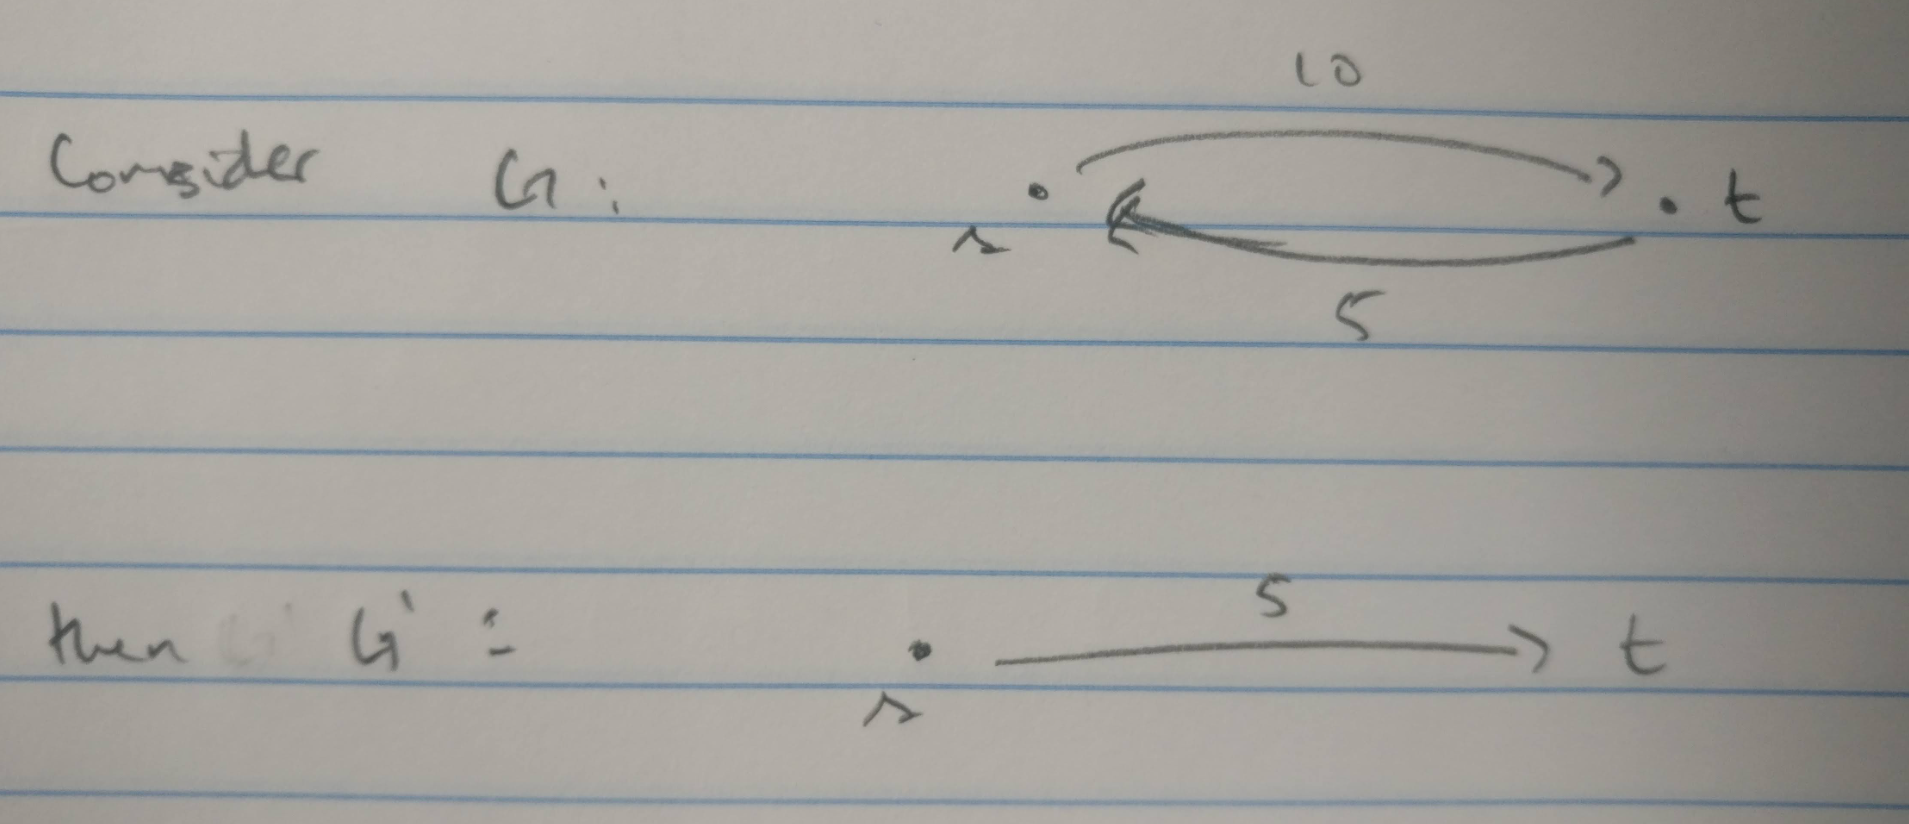
\includegraphics[scale=0.19]{img/7-4-a}
            \caption{Counterexample for statement (a)}
            \label{fig:7-4-a}
        \end{center}
        \end{figure}
    \newpage
    \item Here is a counterexample for statement (b).
    For the min cut in $G$, we have $S = \{ s \} $ and $T = \{ u, t \} $ but for $G'$ I would take $S = \{ s, u \} $ and $T = \{ t \}$.
    Those are the only minimum cuts for their respective graphs and they are not minimum cuts in the other graph.
        \begin{figure}[h]
        \begin{center}
            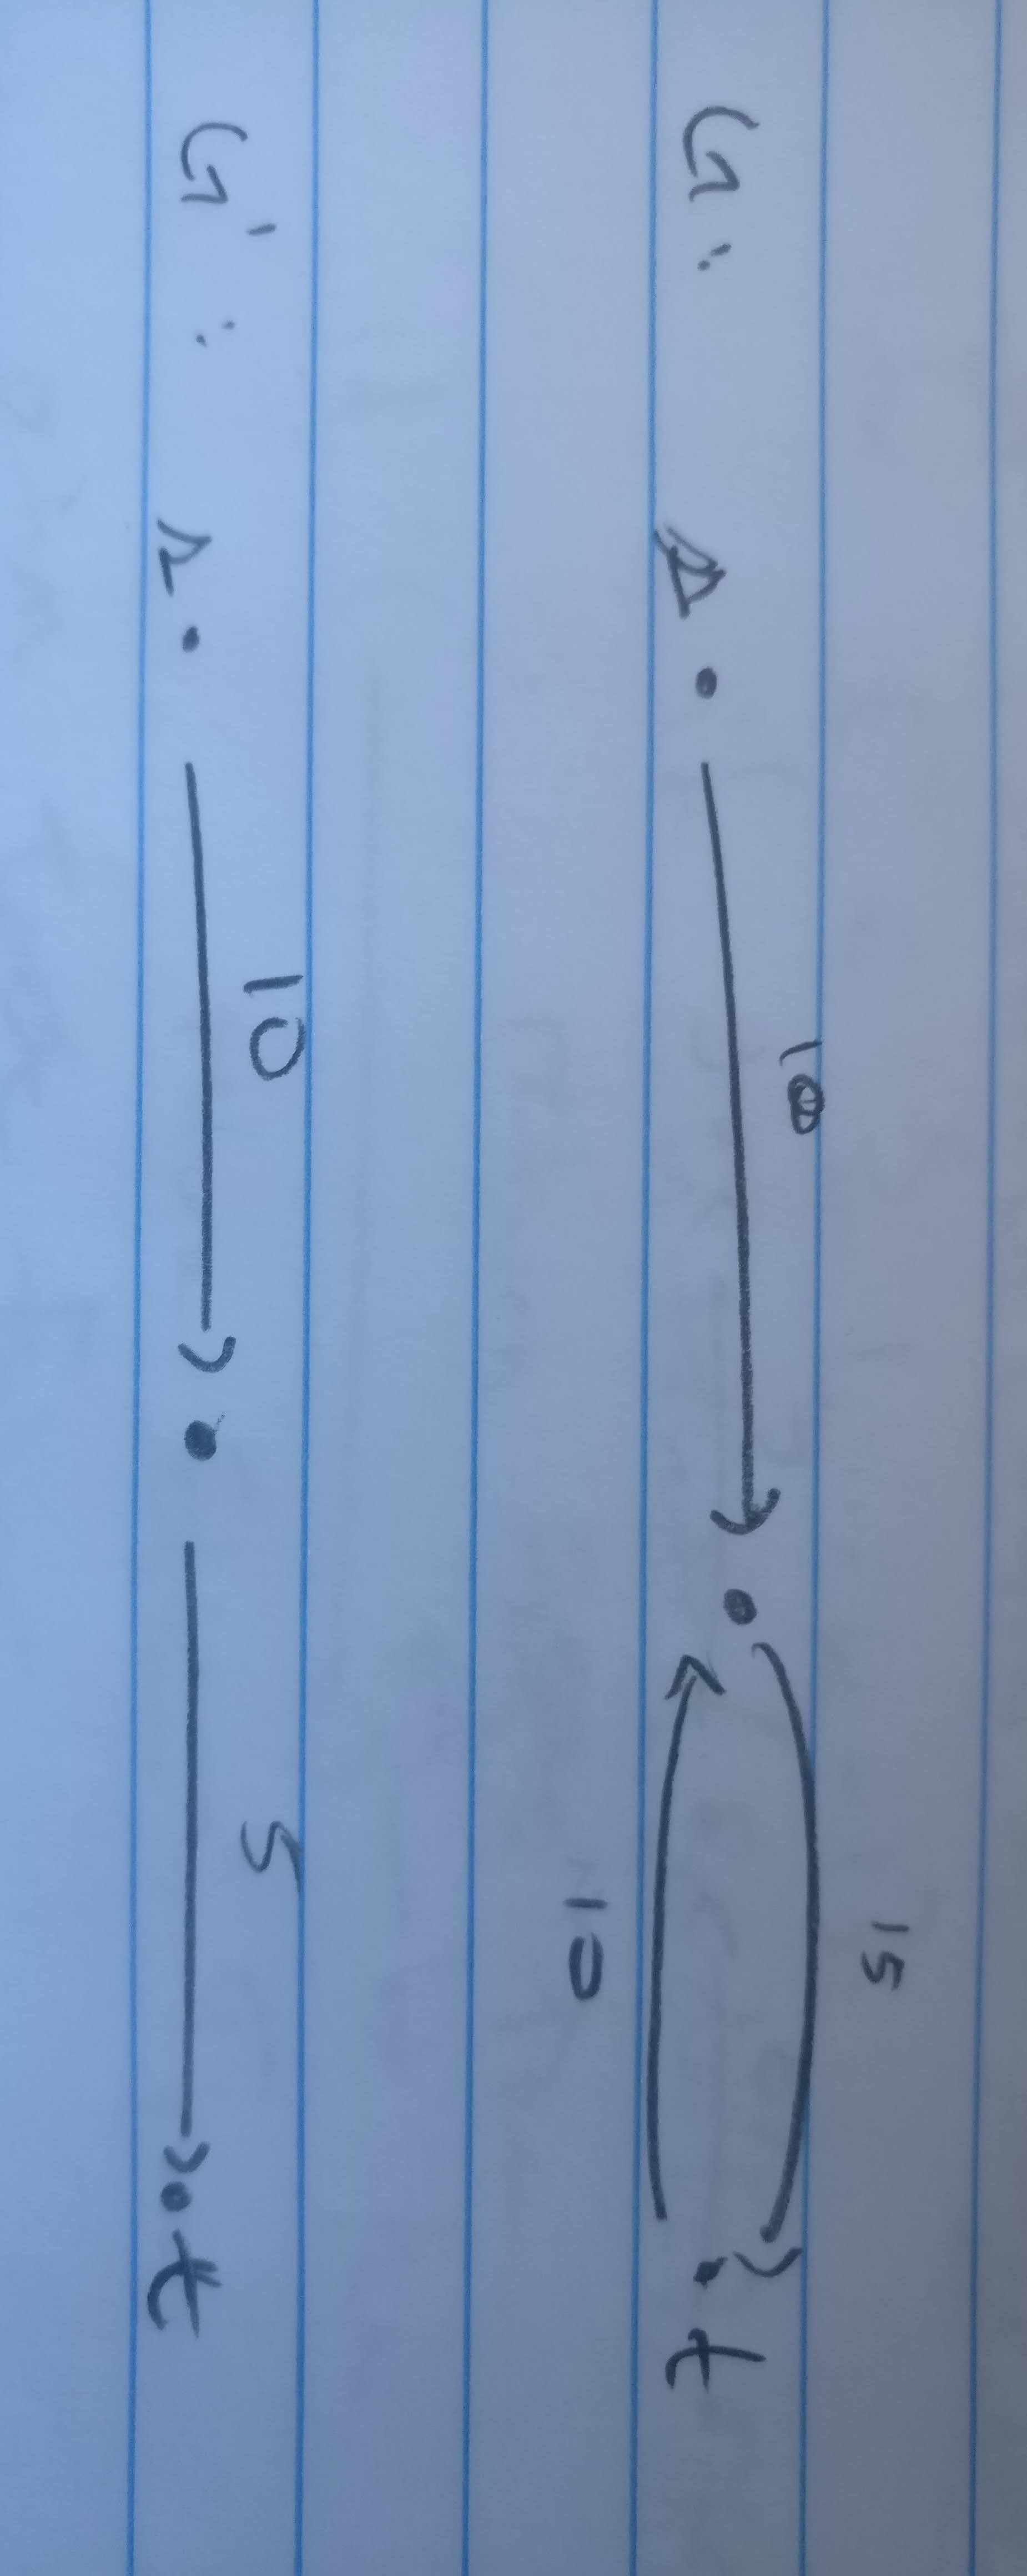
\includegraphics[scale=0.08,angle=90]{img/7-4-b}
            \caption{Counterexample for statement (b)}
            \label{fig:7-4-b}
        \end{center}
        \end{figure}
    \item Here is a counterexample for statement (c).
    The only max flow for $G$ (that does not violate conservation) assigns a flow of 5 to the edges $s \to u$ and $u \to t$ and 0 to all other edges.
    The same max flow exists on the graph $G'$. Since that was the only max flow on $G$ we found a counterexample.
        \begin{figure}[h]
        \begin{center}
            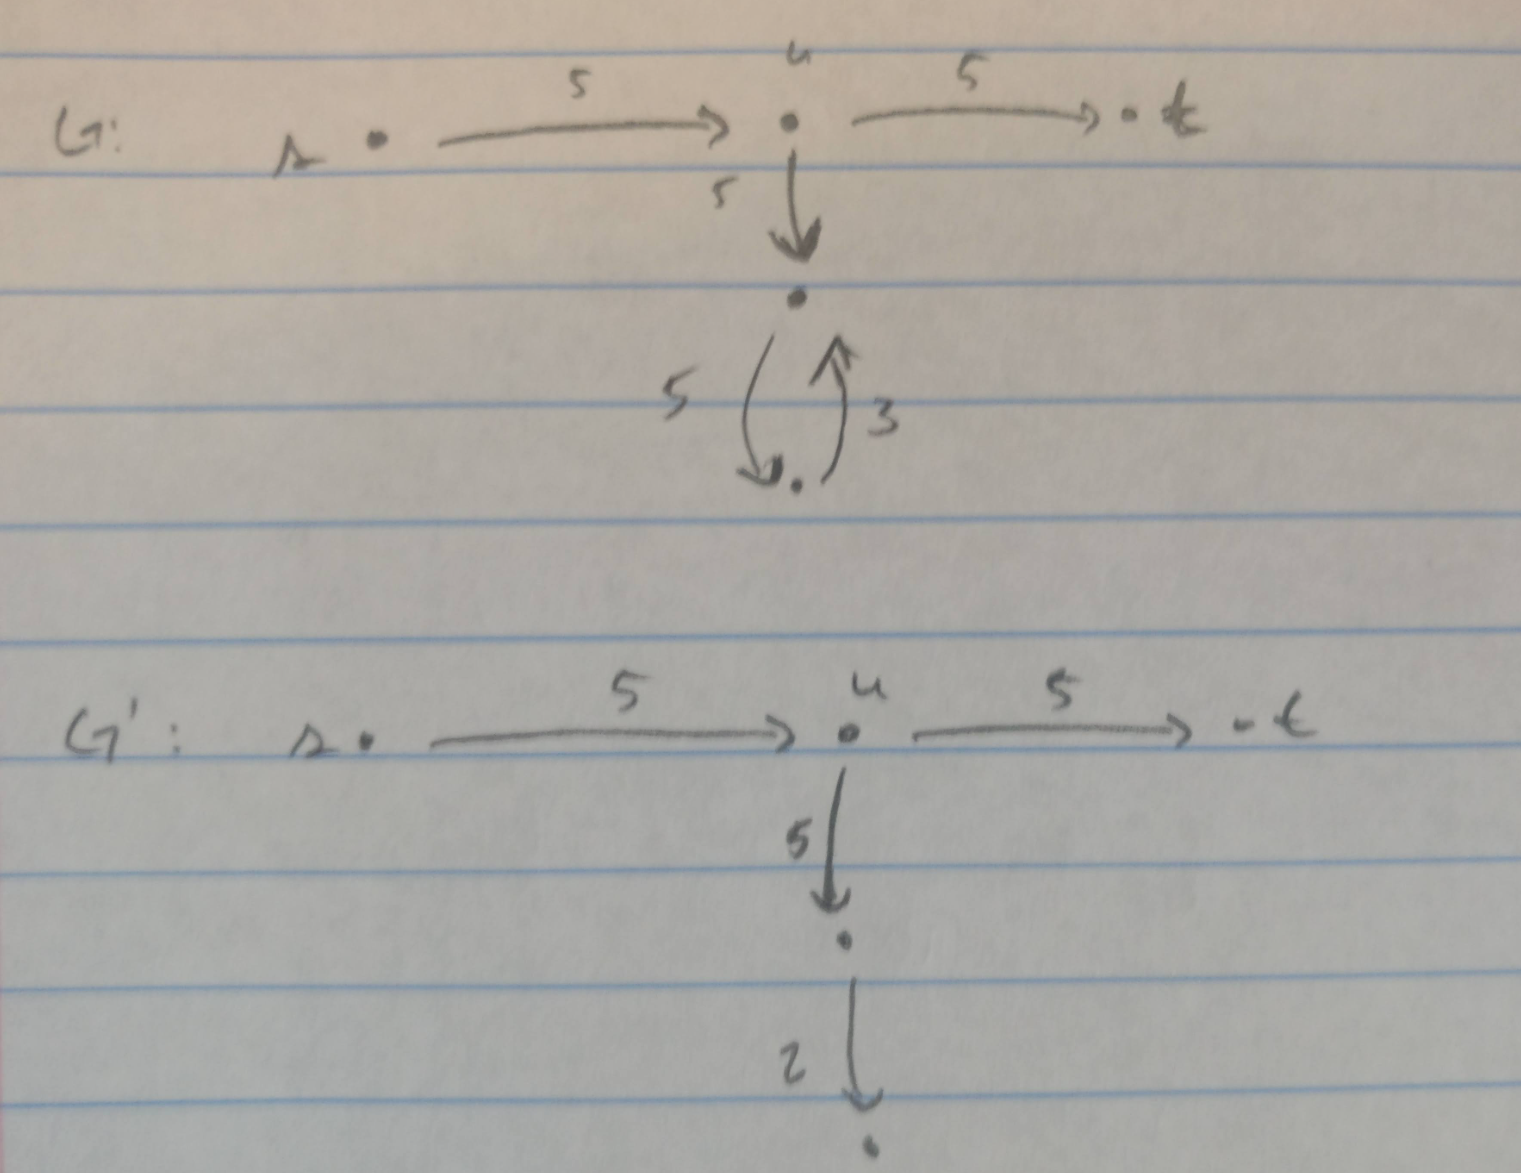
\includegraphics[scale=0.25]{img/7-4-c}
            \caption{Counterexample for statement (c)}
            \label{fig:7-4-c}
        \end{center}
        \end{figure}
\end{enumerate}

% ============================================

\nextprob
\collab{Kevin Browder, Seth Bassetti, Nathan Stouffer}

Chapter 11, Question 6, (Mini-Golf)

The input consists of the $x,y$ coordinates of the $m$ corneres of the playing field, the $n$ starting points, and the $n$ holes.
Every hole can be made in a straight shot from it's starting point.
Assume that you can determine in constant time whether two line segements intersect, given the $x,y$ coordinates of their endpoints.
Describe and analyze an algorithm to compute a one-to-one correspondence between the starting points and the holes that meets the straight-line requirement, or to report that no such correspondence exists.

\paragraph{Answer}

% ============================================

\begin{enumerate}
    \item The goal of this problem is to assign each tee of a mini-golf course to an appropriate hole.
    Each tee can only finish at one hole and each hole must be the destination of exactly only one tee (the assignment of tees to holes is a bijection).
    We also require that each hole can be sunk with a straight shot from the starting point. \parspace
    The mini-golf course is represented as a sequnce of $(x,y)$ pairs stored in an array called $Border[1..b]$.
    We assume that $Border$ is arranged so that the endpoints of lines on the mini-golf course corrspond to the points at consecutive indices of $Border$.
    Additionally we assume that there is a line between the first and last entries of $Border$.
    The final assumption that we make about $Border$ is that connecting consecutive indices with a line forms a closed polygon. \parspace
    The starting points of the course are $(x,y)$ pairs stored in an array called $Tees[1..n]$ and the holes are $(x,y)$ pairs stored in an array called $Holes[1..n]$.
    We assume that $|tees| = |holes|$, otherwise it would be a strange golf course.
    Finally, we assume that every tee and hole has a distinct location inside the polygon formed by the border. \parspace
    The output will be an array called $matches[1..n]$ with $n$ entries.
    The $k^{th}$ element of the $matches$ is an integer representing the hole matched with the $k^{th}$ tee. \parspace
    We assume that we have the following functions $\textsc{Intersect}(p_1, q_1, p_2, q_2)$ and $\textsc{MaxFlow}(G, cap)$.
    $\textsc{Intersect}$ takes in two pairs of points and returns whether the line between $p_1$ and $p_1$ intersects with the line between $p_2$ and $q_2$.
    $\textsc{MaxFlow}$ takes in a graph $G$ and a capacity function $cap$ and uses the Ford-Fulkerson to compute the maximum flow for $G$.
    \item In words, we will solve this problem by forming a special directed graph, solving a max-flow problem on that graph and interpreting the results.
    First, we describe the graph.
    In this graph, the set of vertices is $\{ tee_1, tee_2, ... tee_n, hole_1, hole_2, ..., hole_n, s, t \}$ (one for every tee, one for every hole, and then a source and a target).
    Then, for each $tee_k$, we add an edge to every hole that can be reached with a straight line.
    Then we add an edge from the source vertex to every tee vertex as well as an edge from every hole vertex to the target vertex.
    Every edge is assigned capacity 1. \parspace
    Then we solve the max-flow problem for this graph using the Ford-Fulkerson algorithm and interpret the results.
    If the flow returned from Ford-Fulkerson has capacity less than $n$, then there is no correspondence.
    If the flow returned from Ford-Fulkerson has capcacity $n$ (which is the only other case), then we match each tee with the hole that it sends its flow to.
    \item Here is the algorithm:
    \begin{algorithm}
        \textsc{GolfCourse}($Border[1..b]$, $Tees[1..n]$, $Holes[1..n]$) \\
        1. \hspace{1em} $G = (V,E) \gets \textsc{MakeGraph}(Border, Tees, Holes)$ \\
        2. \hspace{1em} $cap[1..n, 1..n]$   // initialize the capacity function (every entry is 0) \\
        3. \hspace{1em} for $u \to v \in E$ \\
        4. \hspace{2em}     $cap[u,v] \gets 1$ \\
        5. \hspace{1em} $maxflow \gets \textsc{MaxFlow}(G, cap)$ \\
        6. \hspace{1em} if ($|maxflow| < n$) \\
        7. \hspace{2em}     return ``No correspondence'' \\
        8. \hspace{1em} $matches[1..n]$ \\
        9. \hspace{1em} for $u \to v \in E$ \\
        10. \hspace{1.6em} if ($maxflow(u \to v) = 1$ and $u \neq s$ and $v \neq t$) \\
        11. \hspace{2.6em}     $matches[u] = v$ \\
        12. \hspace{0.6em} return $matches$ \\\\

        \textsc{MakeGraph}($Border[1..b]$, $Tees[1..n]$, $Holes[1..n]$) \\
        1. \hspace{1em} $V \gets \{ s, t \} \cup \{ tee_k \}_{k=1}^n \cup \{ hole_k \} _{k=1}^n$ \\
        2. \hspace{1em} $E \gets \{ s \to tee_k) \} _{k=1}^n \cup \{ (hole_k \to t) \} _{k=1}^n $ \\
        3. \hspace{1em} for $k \in \{ 1, 2, ..., n \} $ \\
        4. \hspace{2em}     for $j \in \{ 1, 2, ..., n \} $ \\
        5. \hspace{3em}         if (not \textsc{IntersectBorder}($Border$, $Tees[k]$, $Holes[j]$)) \\
        6. \hspace{4em}             $E \gets E \cup \{ tee_k \to hole_j \}$ \\
        7. \hspace{1em} return $(V, E)$ \\\\

        \textsc{IntersectBorder}($Border[1..b]$, $p_1$, $p_2$) \\
        1. \hspace{1em} for $i \in \{ 1, 2, ..., n-1 \}$ \\
        2. \hspace{2em}     if ($\textsc{Intersect}(Border[i], Border[i+1], p_1, p_2)$) \\
        3. \hspace{3em}         return True \\
        4. \hspace{1em} if ($\textsc{Intersect}(Border[1], Border[n], p_1, p_2)$) \\
        5. \hspace{2em}     return True \\
        6. \hspace{1em} return False
    \end{algorithm}
    \item We prove that our algorithm terminates by showing that it has a finite run time.
    First note that \textsc{IntersectBorder} has a finite run time because it loops over a finite set of natural numbers.
    Also note theat \textsc{MakeGraph} has a finite run time because it is a nested for loop over two finite sets of natural numbers.
    Then the original \textsc{GolfCourse} algorithm has a finite run time.
    \textsc{GolfCourse} it constructs the graph $G$ in finite time on line 1 and has finite loops through line 4 (the number of edges is surely finite).
    Line 5 must be finite because the Ford-Fulkerson Max Flow algorithm runs in finite time.
    Then lines 6-8 are all constant operations.
    Line 9 is for loop over a finite set of edges and line 12 runs in constant time.
    Therefore \textsc{GolfCourse} must have finite run time and terminate.
    \item Proving correctness for this algorithm is different than the rest of the algorithms in this course.
    We proved solved this algorithm with a reduction to max flow, so we will prove that solving the max flow problem on the graph we construct solves the mini golf course problem. \parspace
    We claim that solving the max-flow problem (using the Ford-Fulkerson algorithm) on this graph tells us a way to assign the tees to holes.
    We require the Ford-Fulkerson algorithm so that the flow is an integer-valued function (the integrality theorem from the textbook guarantees integer-valued).
    To verify our claim, note that each tee-vertex can only send out one unit of flow (since it receives exactly one unit of flow from the source).
    Additionally, each hole-vertex can only send out one unit of flow since its only outgoing edge is to the target with capacity 1.
    Then the capacity constraint of a flow forces the flow into each hole-vertex to also be one. \parspace
    Since we are using Ford-Fulkerson, each tee will only be able to send its flow to a single target.
    If the flow returned from Ford-Fulkerson has capacity less than $n$, then there is no correspondence because the maximum flow was not able to reach every tee from the source.
    If the flow returned from Ford-Fulkerson has capcacity $n$ (which is the only other case), then we match each tee with the hole that it sends its flow to and we have a correspondence.
\end{enumerate}

% ============================================

\nextprob
\collab{Kevin Browder, Seth Bassetti, Nathan Stouffer}

Find an algorithm discussed in a recent news article (over the past 12 months).
Choose ONE of the following:
\begin{enumerate}
    \item Look up the primary resource for this algorithm (likely to be a research paper).
    Compare/contrast the similarities and differences between the way the news article describes the problem and algorithm with the way that the primary resource describes it.
    \item If the algorithm itself is not given in the article, provide a prose description of the algorithm along with pseudocode.
    (This might require looking up the primary resource for the algorithm).
    \item Analyze the runtime of the algorithm.
    \item Prove the correctness of the algorithm.
\end{enumerate}

\paragraph{Answer}

% ============================================
	Question: Look up the primary resource for this algorithm (likely to be a research paper).
	Compare/contrast the similarities and differences between the way the news article describes the problem and algorithm with the way that the primary resource describes it.\\
	Answer:
	There were a couple of interesting differences between the news article and the paper. One of the biggest differences I notices was that the article said "the algorithm identified 100\% of COVID-19 carriers confirmed to have the virus but who were not displaying any symptoms" \cite{osborne_2020}. This was slightly misleading because they also had a false positive rate of 16.8\% \cite{9208795}. The way the article phrased it made it seems like they had 100\% accuracy but this was not the case. The article also mentioned that they had 70,000 samples with 2,500 COVID positive individuals. I have no idea where they got the 70,000 number but the paper said they had 2660 COVID positive patients and 27000 controls without COVID. Even if they did have 70,000 samples they could only ever use a little over 5,000 at a time because the positives and controls need to be balanced otherwise the model will skew towards negative as it would be over trained on negatives. \\
	The article also discusses future work that the paper does not go into. The article says the the researcher are working to get more recordings from hospitals to further improve the model. The researchers are also working on a mobile app that integrates the model in an easy to use function. This apparently faces regulatory hurdles that will prevent a quick release.
	

% ============================================


\nextprob
\collab{Kevin Browder, Seth Bassetti, Nathan Stouffer}

Choose an algorithm that you analyzed on a homework in this class (can be this HW or a previous one).
Suppose you are a journalist writing about this break-through algorithm and write a one-page summary of the algorithm for a general audience.
Describing the problem that this algorithm solves and the applications of the problem should be highlighted (feel free to do some research).
Detail of the algorithm and proofs of correctness or runtime should be only given at a very high level.

\paragraph{Answer}

% ============================================
	!!!BREAKING NEWS!!! A group of researchers and students at Montana State University (MSU) in Bozeman, MT have developed an algorithm that matches starting points to holes in mini golf. This is a very important problem because there are many new mini gold course owners who don't know which hole goes with which starting point. This is drastically effecting the times it takes to get their new business running again! Luckily for the owners of the 7,500 mini golf courses in the US there is now a solution. \\
	The team at MSU developed a very clean solution which involves forming a special directed graph and solving a max-flow problem on that graph. From the max flow we can match starting places with holes. If the hole gets max flow from the tee than it is determined that there is a straight shot from tee to hole. The team also realized this was going to stir up a lot of heat in the mini golf world so they proved correctness of the algorithm to nip any controversy in the bud right off the bat. The proved this by demonstrating that if a hole gets full flow from a tee ist must be the associated hole because of the laws of conservation of flow. I love to see them getting ahead of negative press like this. \\
	Beyond the obvious gains to new mini golf course owners, the mini golf course architecture community is a buzz with this new research as well. They will be able to run this algorithm on new designs and determine if a player can get a hole in one at every whole. This is very important to the mini golf pro scene as the pro rules require that a player can achieve a perfect score on a course (by getting a hole in one on every course). \\ The team also released psudocode of their algorithm so it can be easily implemented and used in the mini golf world as soon as possible. There are a few regulatory hurdles that need to be passed before this algorithm can be full released in a commercial form but that should come soon enough! Overall the mini golf world is much better off because of some researchers up in Montana who decided to focus on the great game of mini golf for once instead of just going skiing! 
	
	**Some creative liberties were taken in the writing of this article**
	
	
% ============================================


\newpage

\bibliographystyle{acm}
\bibliography{hw-7}
\end{document}
